\begin{figure*}[!tb]
\centering
%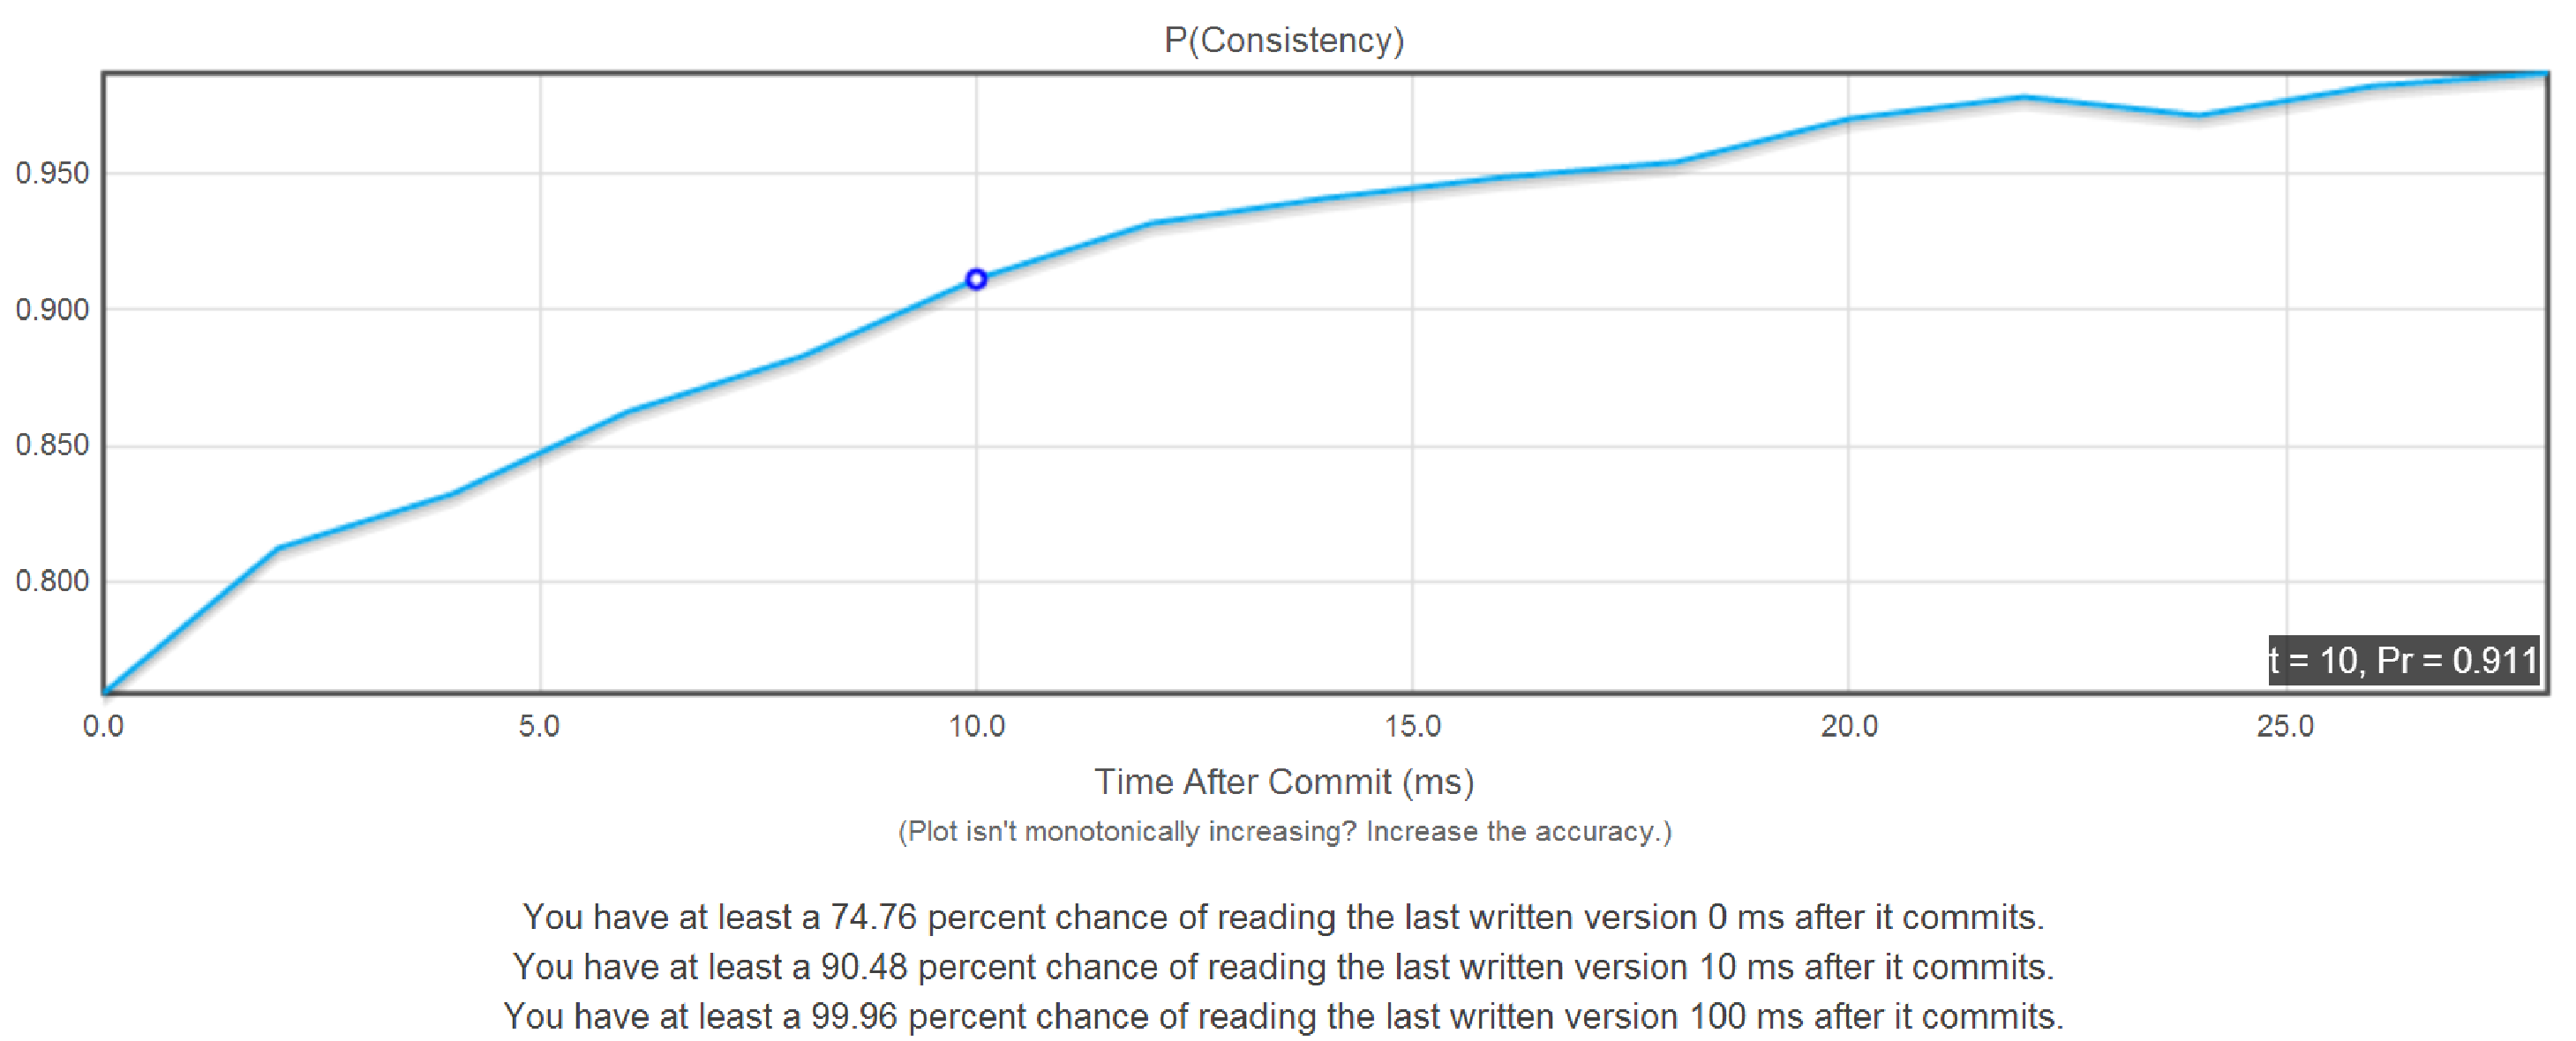
\includegraphics[width=.90\textwidth]{figs/pbs-demo-screenshot.pdf}
\subfigure[Mobile Web App]{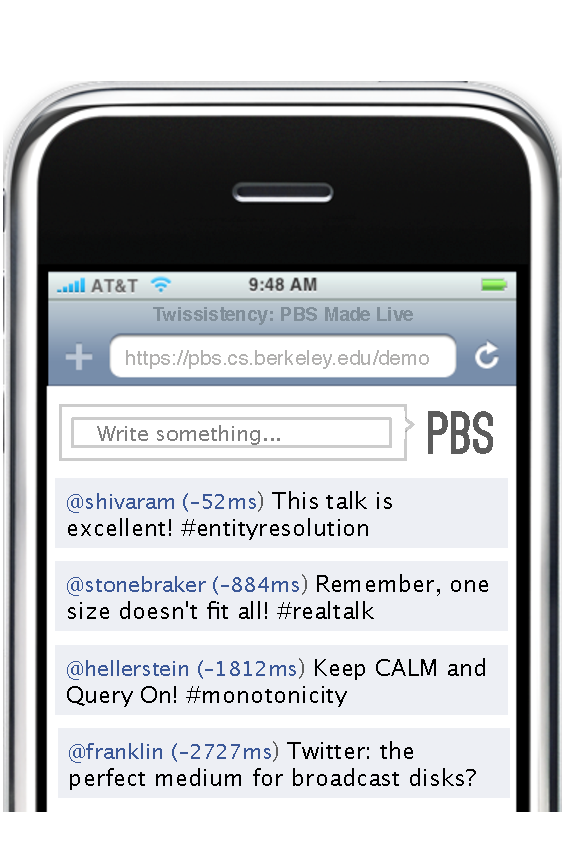
\includegraphics[width=.18\textwidth]{figs/phone.pdf}\label{fig:app}}
\hspace{0.12in}
\subfigure[DBA and Query Tuning Dashboard]{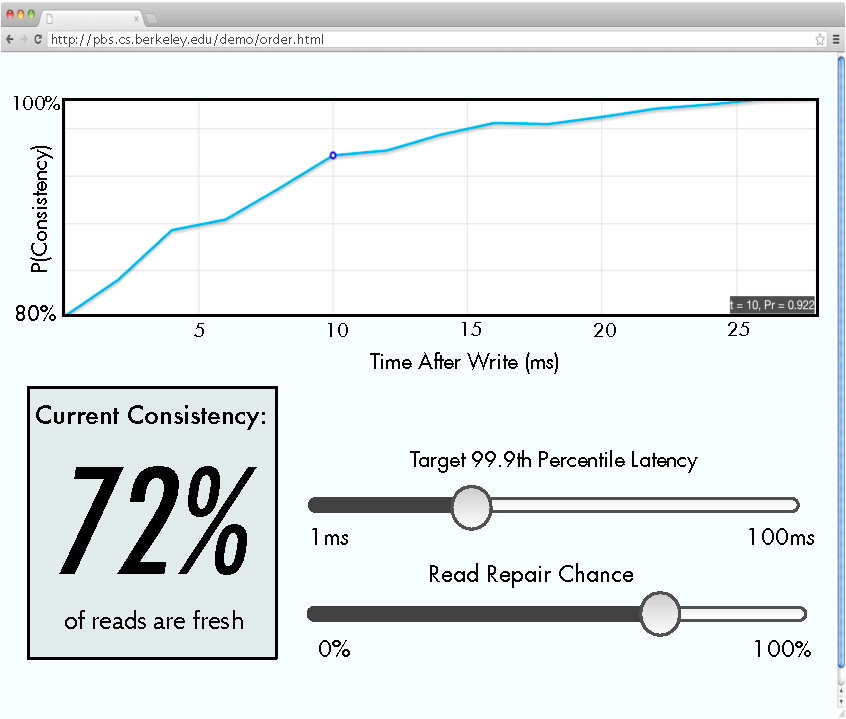
\includegraphics[width=.29\textwidth]{figs/dash.pdf}\label{fig:dash}}
\hspace{0.12in}
\subfigure[Chaos Console]{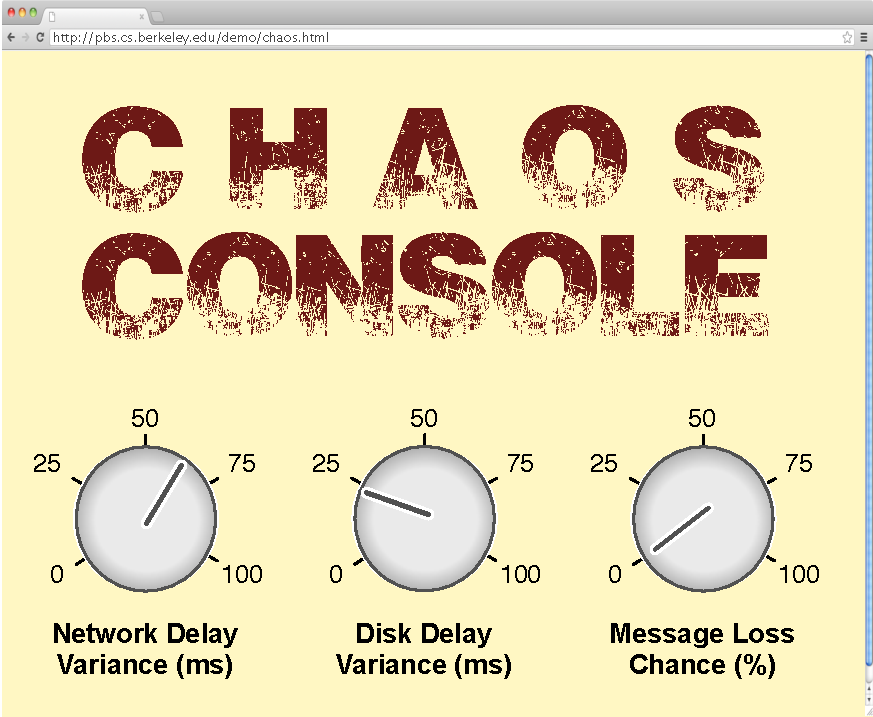
\includegraphics[width=.30\textwidth]{figs/chaos.pdf}\label{fig:chaos}}
\caption{Mock-ups for the mobile social web application---which
  attendees will interact with as end-users---and back-end diagnostic
  views. In the Dashboard, attendees can monitor system consistency
  and set latency and consistency SLAs. In the Chaos Console,
  attendees will wreak havoc on the application's Cassandra cluster
  via several (real-time) configurable failure modes.}
\label{fig:pbs-demo-screenshot}
\end{figure*}

\section{Demo details}
\label{sec:demo}
%Overall theme of the demo and what are goals are: Showing how PBS-metrics can be
%integrated into the DB admin's interface. Also showing why consistency metrics
%are important and how PBS can be used to measure this etc.

At SIGMOD 2013, we will present an end-to-end demonstration that will
show how metrics defined by PBS can be used to improve consistency and
user experience. We will also highlight how database administrators
can monitor and modify system parameters to trade-off consistency for
latency. The demonstration will consist of a user-facing application
and several other components.

%Specific demo setup details: What is the app going to be -- What tables is it
%going to contain and how is this stored in Cassandra ?

As a driving use case, we will implement \textbf{{\systemname}}, a
Twitter-like microblogging application. {\systemname} will expose a
web interface that will be available to all SIGMOD attendees and
provide a mobile application that can be used to post messages about
the conference. In addition to the messages posted by SIGMOD
attendees, we plan to \textbf{replay a corpus} of 4,937,001 Tweets
from conversations obtained from the Twitter firehose between February
and July 2011~\cite{ritter2010unsupervised}. This will help us explore
heavier workloads, particularly in the absence of a deluge of activity
from SIGMOD attendees. {\systemname} will store messages in a
\textbf{Cassandra cluster} running on Amazon EC2. PBS is integrated in
Cassandra, but we will also augment Cassandra to provide consistency
monitoring as described in Section~\ref{sec:dbarch}.

%Demo screens detail - We will have two screens and what each one will show. How
%can the audience interact with the demo ?

To illustrate the utility of consistency metrics, we will provide
attendees with the opportunity to experience consistency from three
perspectives: as user, administrator, and powerful adversary.

The \textbf{user interface} screen will host the {\systemname}
front-end and will allow attendees to post and read messages
(Figure~\ref{fig:app}). We will also provide a setting that
allows users to see how old messages are and manually inspect the
end-to-end delay for each message. %from the write to their chosen interface.

To provide the experience of a database administrator or operations
technician, we will have a \textbf{monitoring and control console}
that measures and plots the consistency and latency over 10-second
time intervals (Figure~\ref{fig:dash}).
%\footnote{We previously
%released an interactive, browser-based demo online at
%\url{http://pbs.cs.berkeley.edu/#demo} (but did not officially
%demonstrate it in a peer-reviewed forum). We expect to build a
%similar prototype for the first portion of the monitoring console
%design. However, the online demo is based on synthetic data, while
%the proposed demo runs in real-time on a real cluster.}
Additionally the interface will allow users to modify system parameters like
the read repair chance and set consistency SLAs for read and write
operations. We will change the system parameters in real-time, and the
consistency SLAs will affect all users' actions on the site
%---both from the replay stream and attendees accessing {\systemname}.

Consistency is particularly interesting under changing environmental
conditions, so we will allow participants to control parameters like
system latency and the performance of several replicas. We will provide
a \textbf{chaos console}, a separate interface that can be used to
inject message delays, model message loss, and artificially
slow Cassandra instances to demonstrate their effect on consistency
(Figure~\ref{fig:chaos}). We will physically implement the actual failures via
both JVM manipulation and host-based kernel operations. In addition to
improving engagement, this will allow attendees to both induce
consistency anomalies and understand the impact of several common
failure modes.
